\documentclass[english,10pt,a4paper,oneside,twocolumn,titlepage]{report}
\usepackage[utf8]{inputenc}
\usepackage[T1]{fontenc}
\usepackage[width=17.00cm, height=23.00cm]{geometry}
\usepackage{babel}
\usepackage{amsmath}
\usepackage{algorithm}
\usepackage{amssymb}
\usepackage{graphicx}
\usepackage{subfigure}
\usepackage{algpseudocode}
\usepackage{tikz}
\renewcommand{\thesection}{\arabic{section}}

\title{Notes on Pyrolysis Material Study}
\author{Vincent Le Maout}
\begin{document}
	\maketitle
	
	%-----------------------------------------
	\section{Introduction}
	\label{section0}
	These notes intend to progressively introduce the
	reader to the physics commonly adopted to describe 
	ablative materials for Thermal Protection Systems 
	(TPSs) in the literature. Commonly used for 
	very high speed reentry in aerospace industry, they
	are highly studied as the sizing of the TPSs is 
	currently one of the bottleneck for increasing the 
	payload for space exploration. \\ 
	This class of material have to be distinguished from 
	passive materials, that only store incoming energy and
	are used as heat sink, but can be re-used several times,
	 and actively cooled materials, which benefits from local
	 heat dissipation to mitigate the incoming heat flux. On 
	 the other hand, pyrolising TPS are employed for their
	 high potential in limiting the transport of energy in depth
	 of the space vehicle, at the expanse of self-degradation 
	 due to surface and in-depth heterogeneous reactions
	  under high temperature, preventing their 
	  employ for future mission.
	 This degradation process leads to an expel of energy 
	 due to out-gassing of hot products resulting from
	  material	 ablation out of the vehicle. Eventually, the 
	 underlying surface blowing is increasing the 
	 thickness of the boundary layer, mitigating further
	 convective heating in complex multi-physics processes.
	 This will not be considered in these notes.	 \\
	 All the presented models derived thereafter
	 are already implemented in the open source 
	software PATO, and all the presented examples 
	have been obtained using it. 
	Starting from a simple heat transfer problem, the 
	specificity of pyrolysing materials will be progressively 
	introduced, and examples will provide an overview 
	of the sensitivity of the results regarding the 
	multiple physical processes at play within TPSs during
	atmospheric reentry. Finally, a note on ablation process
	and its effects on in-depths energy transport will close 
	this note. The main literature sources used to write these
	notes are the following: \cite{Lachaud2017}, 
	\cite{Marschall2015} and \cite{Johnston2014}.

	%-----------------------------------------
	\section{TPS Physical Modelling}
	\label{section1_0}
	In this section, the physics of ablative materials is 
	described step by step by starting from a simple heat
	 conduction problem
	that will serve as a reference as it is the behaviour of 
	passive TPS. As the problem may be seen by some
	as artificial, the readers already familiar with the topic are 
	encouraged to look directly at the main references used 
	for these notes. Finally, for readers more interested by 
	surface and mass balance between the TPS and the 
	boundary layer, the topic is addressed in section 
	\ref{section2_0}.
	\subsection{A Simple Conduction Problem}
	 \label{section1_1}
	 Let's start by considering a material submitted to a 
	 time independent imposed temperature on one end, 
	 whereas the other is considered adiabatic
	 (see Figure \ref{figure1_1}).  The imposed temperature 
	 is chosen to be representative of temperature usually 
	 encountered over TPS surface such as it is expected it 
	 will trigger pyrolysis in the future
	\begin{figure}[h]
	\centering
	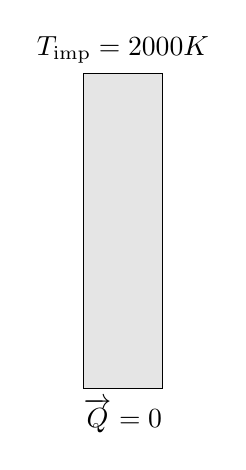
\begin{tikzpicture}[scale=2]
	\filldraw[color=gray!20, draw=black]
  	(0, 0) -- (0, 2) -- (0.5, 2) -- (0.5, 0) -- cycle;
  	%\draw[->, color=red] (0.0, 2.5) -- (0.0, 2.01) ;
  	%\draw[->, color=red] (0.25, 2.5) -- (0.25, 2.01) ;
  	%\draw[->, color=red] (0.5, 2.5) -- (0.5, 2.01) ;
  	\draw (0.25, 2.) node[above]{$T_{\text{imp}} = 
  	2000K$} ;
  	\draw (0.25, 0) node[below]
  	{$\overrightarrow{Q} = 0$} ;
	\end{tikzpicture}
	\caption{\label{figure1_1} Schematic of the 
	configuration studied in the next section.}
	\end{figure}
	 If the material is assumed to be non porous such
	 as passive materials, the description of energy transport
	 is generally assumes to follow the Fourier law which
	 reads as :
	 \begin{align}
	 \frac{\partial }{\partial t} \left(\rho^s c_p^s T^s \right)
	 - \nabla \left( \lambda^s \nabla T^s \right) &
	  = 0 \label{energy_1} \\
	  \frac{\partial }{\partial t} \left(\rho^s  \right) &
	  = 0  \label{mass_1} 
	 \end{align}  
	 The upper script $^s$ denotes solid phase related
	 properties. In the future, for porous material, the 
	 upper script $^g$ will be used for gas phase related
	 variables. Additionally, it is assumed for now that
	 the solid material is homogeneous, \textit{i.e.} made
	 of only one pure phase such as steel or carbon graphite.
	 However, the reader should keep in mind that in the
	 next parts, the composite nature of the TPS will be 
	 introduced, and the different solid phases will be 
	 indexed as $^{s_1}, ^{s_2},  ..., ^{s_n}$ following the
	 notation in \cite{Marschall2015}. 
	 In equation \eqref{energy_1}, the assumption of solid 
	 material energy $e^s = c_p^s T^s$ has been made.
	 Equation \eqref{mass_1} translates the fact that for
	 a non porous material, there is no variation of material
	 density \textit{a priori}. 
	 Any phase change or heterogeneous chemical 
	 reactions are 
	 happening at the boundary (the material being \textbf{
	 non porous}, no volumetric chemistry is considered) and
	 only surface ablation can be considered in such 
	 configuration (see section \ref{section2_0}). 
	 
	 An example of simulation with this kind of material is
	 shown on Figure \ref{figure1_2}. In this example, for 
	 the sake of simplicity, the material properties $c_p^s$ 
	 and $\lambda^s$ has been chosen constant and are 
	 reported on Table \ref{table1_1}. In that configuration, 
	 an analytical solution exists \cite{Hahn2012}
	 
	 It can be noted that
	 as previously said, this example is artificial in the sense
	 that there are currently no dissipative processes 
	 occurring on the top boundary of the numerical
	 domain. Consequently, surface temperature 
	 keeps increasing whereas in reality :
	 \begin{itemize}
	 \item Radiative cooling would \textbf{bound}
	  the surface 
	 temperature, preventing it from reaching such a high 
	 value. This cooling is the most efficient one (as it scales
	 with the fourth power of surface temperature, see 
	 section \ref{section2_0}), but additional local dissipation
	 processes would also intervene in reality (melting,
	  sublimation...)
	  \item The surface heat flux is directly provided by the 
	  thermal state of the boundary layer. The use of a 
	  \textbf{constant} non-homogeneous 
	  Neumann boundary 
	  conditions is physically irrelevant, as the effect of
	  convective heating over the material is reduced as 
	  surface temperature rises (let's consider for example
	  a simple Newton's approximation for boundary layer
	  heat flux of the form $ \overrightarrow{Q}
	   = \alpha \left(T^g_{e} - T^s_{s} \right) $ 
	   with $T^g_{e} $ the \textbf{gas
	  phase} boundary layer edge temperature and $T^s_{s}
	  $ the \textbf{material} surface temperature. Ultimately, 
	  as material surface temperature becomes hotter than
	  the boundary layer, the heat flux sign would reverse, 
	  and the fluid would cool down the surface.
	 \end{itemize} 
	
	%-----------------------------------------
	\section{Surface Balance for TPS}
	\label{section2_0}
	Now that the physics at play inside ablative material have
	been (more or less) uncovered, the attention of the 
	reader is drawn on the surface specific processes whose 
	consequences results in the self-degradation of ablative
	material as discussed in the previous section 
	\ref{section1_0}.

	%----------------------------------------
	\pagebreak
	\appendix

	
	%-----------------------------------------
	% my bibliography
	\bibliography{mybliblio}
	\bibliographystyle{ieeetr}
	
	
\end{document}

